\chapter{Caso 2: Anti}

% Este apartado puede convertirse en un artículo por sí mismo. Describirlo de una manera distinta al tipo contexto, planteamiento, proceso y resultados  

% \href{https://anti.ocelotl.cc}{\includegraphics[width=\textwidth]{img/anti01.png}} % Una imagen que también es hipervínculo 

\begin{figure}[tb]
\centering 
\includegraphics[width=\columnwidth]{../../img/anti01.png} 
\caption[Captura de Anti]{Captura de anti y de la interfaz gráfica que utiliza de \url{https://anti.ocelotl.cc}.} % The text in the square bracket is the caption for the list of figures while the text in the curly brackets is the figure caption
\label{fig:gallery} 
\end{figure}

% Anti es una pieza que parte de la ofuscación para plantear una reflexión sobre la relación que existe entre usuarios y tecnología. Utiliza algunos módulos de \gls{aprendizajeautomatico} (machine learning) 

%\subsection{Contexto}

\iftoggle{tesis}
{La ofuscación puede definirse como el acto deliberado de encubrir el significado de una comunicación. Para el caso de la programación y apuntando ideas hacia los estudios del software, la presente investigación toma la noción de ofuscación de un conjunto de posibilidades para la escritura de software que coinciden, dialogan o se enfrentan a que podríamos definir como la convención de la \emph{estética del código} y aquellos programas que exploran ``otros principios estéticos'' además de los convencionales.

Edsger Dijkstra conoincide con la delimitación convencional de esta forma de escribir programas:

\begin{quote}
``[..] el programador no difiere de algún otro artesano: a menos de que ame sus herramientas, es altamente improbable que pueda crear algo de calidad superior. Al mismo tiempo estas consideraciones nos hablan de las más grandes virtudes que un programa puede mostrar: Elegancia y Belleza''\citep[p.~10]{EWD:EWD35}
\end{quote}

Como respuesta a la posición de Dijkstra y en un ámbito de programación que se aproxima lúdicamente a la escritura de programas, la ofuscación:

\begin{quote}

`` arroja luz a la naturaleza del código fuente, que es leído por un humano e interpretado por una máquina, y puede recordar a los críticos la búsqueda por diferentes dimensiones de sentido y múltiples codeos en todo tipo de programas''\citep[p.~198]{obfuscatedCode}

\end{quote}

El código su lectura, así como las funciones de los programas que ejecuta, son subjetivas y están determinadas por un sentido imputado que socialmente se acuerda de manera tácita y que puede ser visibilizado para interpelarlo en un sentido crítico, lúdico e incluso satírico.\footnote{Tal es el caso de Windows 93 del artista Jankenpopp. \url{https://www.windows93.net/} } En este punto encontramos conexiones con las posibilidades de la programación en una dimensión artística:

\begin{quote}
``[La práctica de la programación ofuscada] sugiere que el codeo puede resistir a la claridad y a la elegancia para pugnar en su lugar por la complejidad, puede hacer familiar lo desconocido y puede luchar con el lenguaje en el que está escrito, justo como lo hace la literatura contemporánea.''\citep[p.~198]{obfuscatedCode}
\end{quote}}
{La ofuscación puede definirse como el acto deliberado de encubrir el significado de una comunicación. Para el caso de la programación y apuntando ideas hacia los estudios del software, la presente investigación toma la noción de ofuscación de un conjunto de posibilidades para la escritura de software que coinciden, dialogan o se enfrentan a que podríamos definir como la convención de la \emph{estética del código} \citep{EWD:EWD35} y aquellos programas que exploran ``otros principios estéticos'' \citep{obfuscatedCode} además de los convencionales.}

¿Puede el código fuente ``luchar'' en contra del marco de uso para el que fue escrito?

% Para la versión expandida podría citar las referencias 

%% En este punto puedo retomar las ideas de djisktra y de knuth 

Esta definición es el punto de partida de \emph{Anti}, una pieza audiovisual para el navegador que tiene dos objetivos: visibilizar la discusión en torno a el uso de datos y la responsabilidad tecnológica del usuario y 2) actuar como un dispositivo de ofuscación facial y vocal que pueda utilizarse en situaciones de uso cotidiano. 

El maquillaje y el uso de accesorios anti-vigilancia son estrategias analógicas para evitar la detección de rostros. En una situación de protección fuera del entorno digital, incluso una máscara de leds puede cumplir esta función.

El presente proyecto se enfoca los mecanismos de anti-vigilancia que pueden realizarse de manera digital, teniendo a la computadora como un agente intermedio entre dos puntos que desean mantener algún tipo de comunicación gestual y vocal sin que estos puedan detectarse o asociarse a sujetos específicos, sin que esto implique que la comunicación sea completamente ofuscada para los usuarios.

% En la versión extendida para la tesis, aquí va el apartado de puesta en marcha y montaje. Considero que para el artículo puede ser innecesariamente extenso



\section{Delimitación y contexto}


Inicialmente la aplicación fue concebida para ser ejecutada localmente. Dadas las circunstancias específicas de la pandemia de COVID-19, el proyecto migró a una aplicación web.

Una de las consecuencias no buscadas del desarrollo para la web fue la compatibilidad entre sistemas operativos y la cero instalación de entornos y librerías; la aplicación puede ejecutarse con un navegador web actual 

La pieza está alojada en la web y utiliza tone.js como motor de audio y three.js para el despliegue de gráficos tridimensionales. Adicionalmente utiliza: 1) Tensorflow.js para la lectura de puntos de referencia faciales (face-landmark-detection) y 2) algunos módulos adicionales de la librería JSM para el rendereo de efectos de post-proceso de imagen.

\iftoggle{tesis}
{\subsection{Esquema general de la aplicación}}

La aplicación cuenta con tres momentos principales: 1) Detección de puntos de referencia faciales 2) motores gráfico y sonoro, 3) materiales y organización y 4) Redirección de flujos de audio y sonido.



\subsection{Puesta en marcha y montaje}

Anti es una obra que aprovecha las posibilidades de la interactividad en la producción artística con nuevos medios. En este sentido, la relación de la pieza con el especttador coincide con el planteamiento de Hugo Solís que define a esta relación como:

\begin{quote}

``arte que requiere de un input directo por parte de los espectadores para poder considerarse una obra terminada y funcional. Hablamos de obras no lineales en donde al menos uno de los elementos resultantes, comúnmente observable, dependerá de la información que proviene del espectador, directa o indirectamente, ya sea presencial, o remotamente en el momento de la observación, o anticipadamente.''\citep[p.~37]{hugoSolis}

\end{quote}
  
Anti tuvo una modalidad de exhibición presencial que tuvo lugar en el Antiguo Colegio de San Ildefonso. Uno de los problemas del montaje en modo exhibición tuvo que ver con el acceso a internet. Una de las problematizaciones más importantes de la pieza tuvo que ver con la circulación de planteamientos sobre la cultura libre en el espacio público. Una pregunta importante que queda en el aire se relaciona directamente con el acceso tecnológico a sitios, piezas, informaciones y conocimientos que se expresan a través de la web. La posibilidad de acceder a estos espacios digitales queda restringida por una infraestructura que queda limitada en el contexto de un país latinoamericano con el acceso m+as cercano a los nodos internacionales de acceso a internet del mundo. 

\begin{figure}[tb]
\centering 
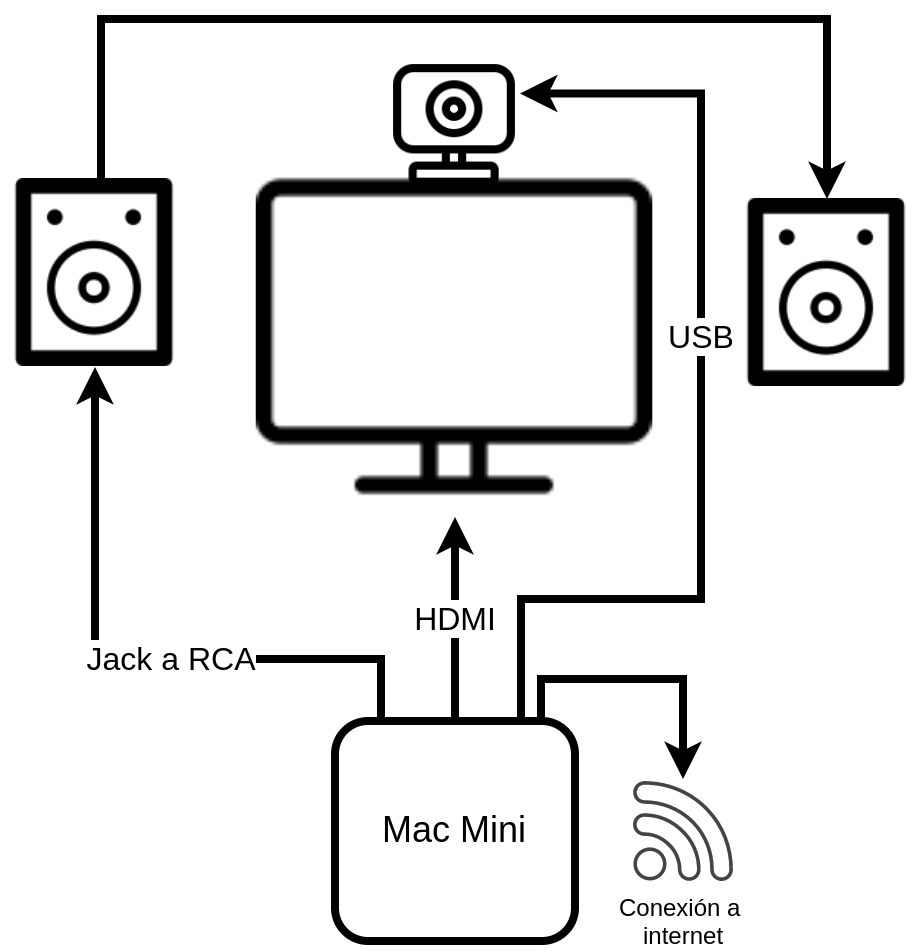
\includegraphics[width=0.7\columnwidth]{../../img/antiExWhite.png} 
\caption[Diagrama de Montaje Anti]{Diagrama de montaje de Anti.} % The text in the square bracket is the caption for the list of figures while the text in the curly brackets is the figure caption
\label{fig:gallery} 
\end{figure}

\begin{figure}[tb]
\centering 
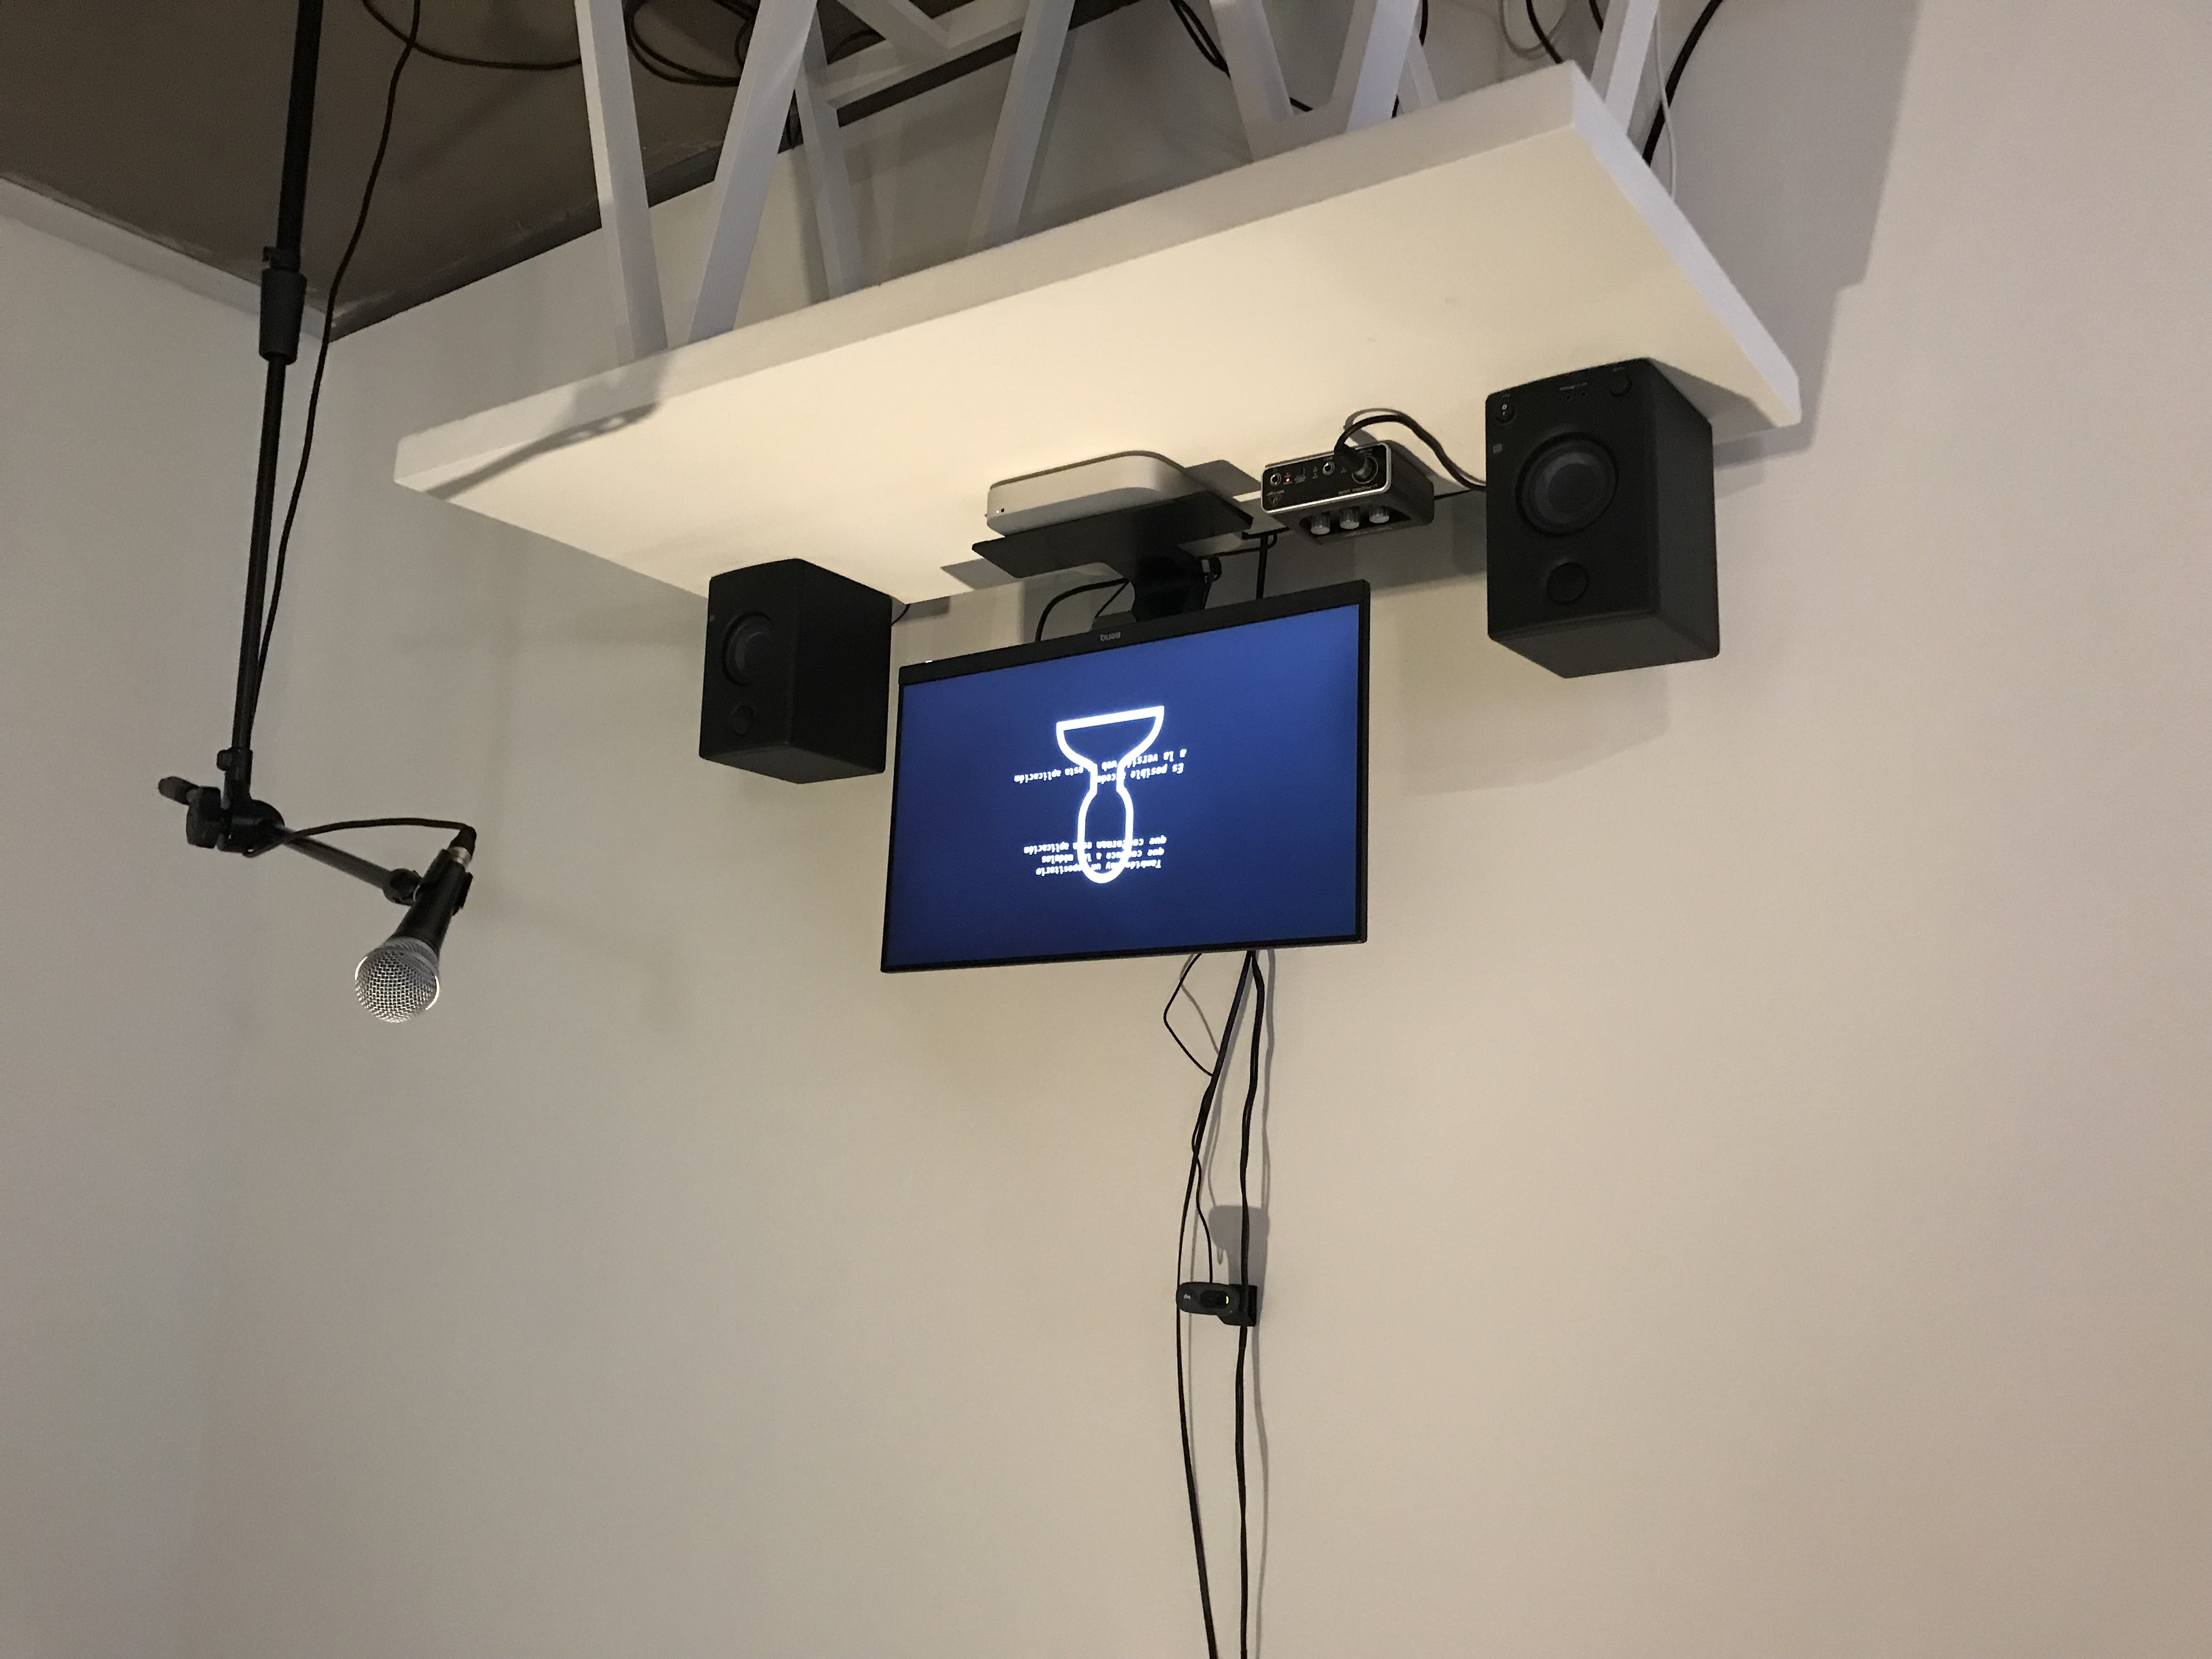
\includegraphics[width=\columnwidth]{../../img/ildefonso.jpg} 
\caption[Montaje Anti en San Ildefonso]{Montaje final en el Antiguo Colegio de San Ildefonso} % The text in the square bracket is the caption for the list of figures while the text in the curly brackets is the figure caption
\label{fig:gallery} 
\end{figure}


\subsection{Ecosistema}

Documentación de las piezas que compartieron tiempo y espacio con anti. Preocupaciones compartidas por las consecuencias sociales de la tecnología y el uso responsable de éstas para transformarla, de acuerdo a lo que se mencionó anteriormente de Soon y Cox. Contexto de la desapariciones de los feminicidios en México, la contaminación provocada por el consumo de fast fashion y la relación / interpretación de la realidad a partir de narrativas que contemplan la agencia no-humana. 

La centralidad del individuo 

La idea de múltiples programas de los objetos tecnológicos \citep{latour}

%\section{Descripción técnica general}

Precisión 

\section{Audio e Imagen} % Relevante o puede ir en otro apartado? 

El uso de motores gráficos y de audio decidió el rumbo de la aplicación. Hasta el momento hay dos versiones del proyecto:

\begin{enumerate}

\item La primera versión inicializó el trabajo con recursividad y ejecución de audio por medio de secuenciadores sencillos escritos en Tone.js
\item La segunda versión incorporó a Hydra como una librería externa para la renderización de texturas que pudieran adecuarse a las posibilidades de ofuscación de la capa que \emph{complejizaba} la lectura del rostro
\item Tentativamente la tercera versión se desplazará del entorno de renderización Hydra para explorar las posibilidades de la generación de texturas por medio de shaders.
  
\end{enumerate}

\subsection{Audio}

¿Por qué Tone.js? 

\subsection{Imagen}

¿Por qué Three.js?
keypoints y la construcción de meshes > triangulaciones y las convenciones del modelado tridimensional 

Hydra como un módulo para generar texturas en sólidos 

%\subsection{Redirección de flujos de audio y sonido}

\section{Eventos}

\subsection{Puntos y desarrollo}

El desplazamiento del evento musical y la diversificación de los materiales. Peculiaridades del texto, sonido e imagen. Eventos que establecen puntos de salida y de llegada. Preguntas sobre lo que existe entre puntos. La rampa de tiempo como una forma de relacionar eventualidades y desarrollarlas en el tiempo.

\subsection{Transducción de magnitudes}

Relaciones y diferencias. Transducción de magnitudes 

La biblioteca MediaPipe Facemesh devuelve 468 puntos de referencia faciales. ¿Cómo estos puntos son relevantes? 

Promedios de movimiento asociados a todo y a regiones del rostro. 

\subsection{Materiales}

%\subsection{Materiales y organización}

En esta parte se distribuyeron los materiales sonoros, visuales y textuales en eventos que pudieran detonarse a partir de un esquema temporal y espacial a manera de partitura. 

Texturas

\section{El tiempo en el navegador}

\subsection{Tiempo y secuenciación}

Este apartado puede hablar de las diferencias que existen entre las distintas formas de transformar eventos en el tiempo: setInterval, requestAnimationFrame, Tweenjs y los objetos de Tone.js que permiten detonar eventos como si fueran secuenciadores. Hasta el momento se han detectado tres tipos de aproximaciones: 1) Aquella que está medida en microsegundos y que no necesariamente es precisa, 2) aquella que tiene que ver con temporalidades medidas en segundos ( de hecho el diseño de la estructura general de la pieza tomó esta división con punto de partida y 3) la aproximación que coincide con la convención musical basada en golpes por segundo (BPM). 

\subsection{Panorámica}

Partitura

\begin{figure}[tb]
\centering 
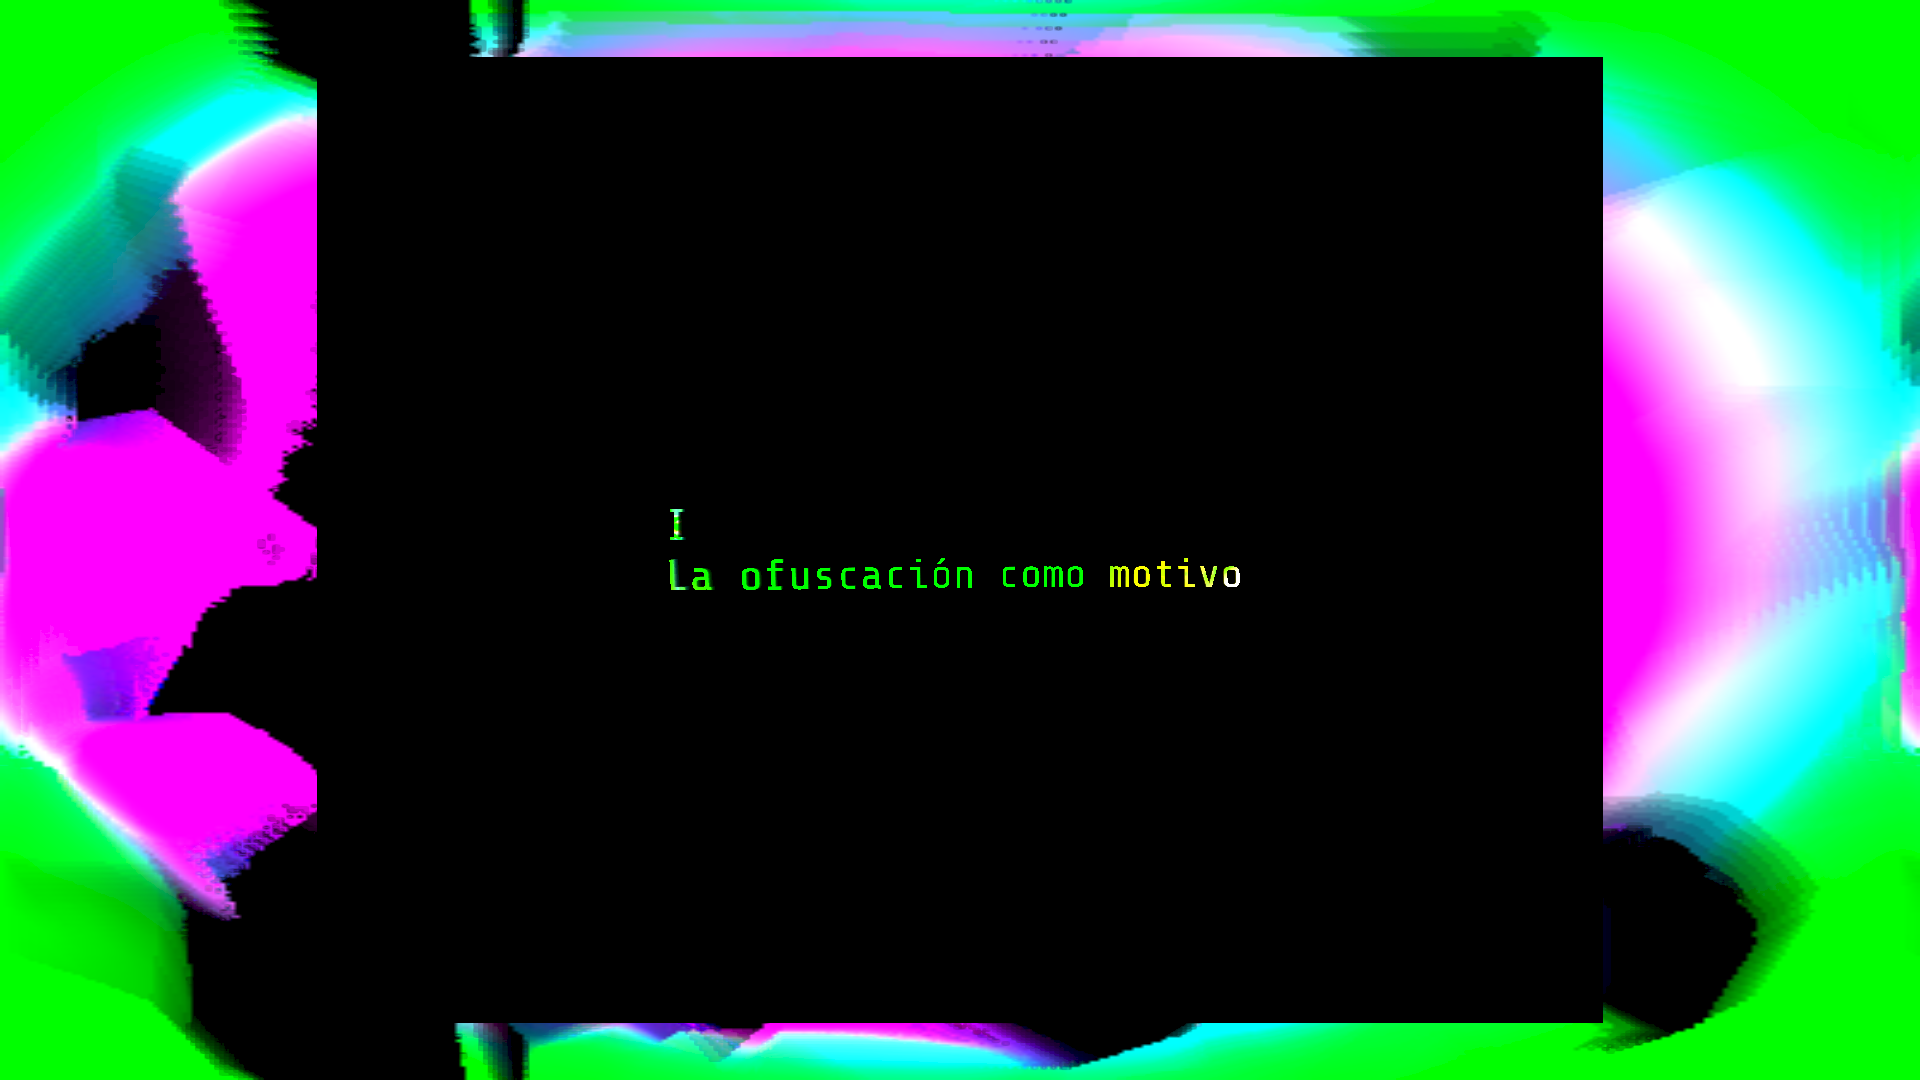
\includegraphics[width=\columnwidth]{../../img/antiHydra1.png} 
\caption[Título 1]{Primer título de anti}
\label{fig:gallery} 
\end{figure}

\section{La ofuscación como motivo}

\subsection{Predicciones}

Anti utiliza la biblioteca MediaPipe Facemesh\footnote{MediaPipe Facemesh un un paquete ligero que predice 486 puntos faciales tridimensionales para inferir la superficie geométrica aproximada de una cara humana. Consultado el \today en: Nota: esperar a que suban el paquete} para la detección de puntos de referencia faciales. Estos puntos están optimizados para que las zonas de la cara con mayor gestualidad tengan una densidad de puntos mayor. \citep{kartynnik2019realtime}.

\subsection{Ofuscación audiovisual}

Aquí podría hablar de los aspectos tecnológicos que motivaron la realización de la pieza. Tecnologías diversas que pueden coincidir (no necesariamente lo hacen, por lo menosen términos de la declaratoria y motivación de los proyectos) con la ofuscación facial. Tensorflow y face-landmark-detection. 
te

\begin{figure}
\centering 
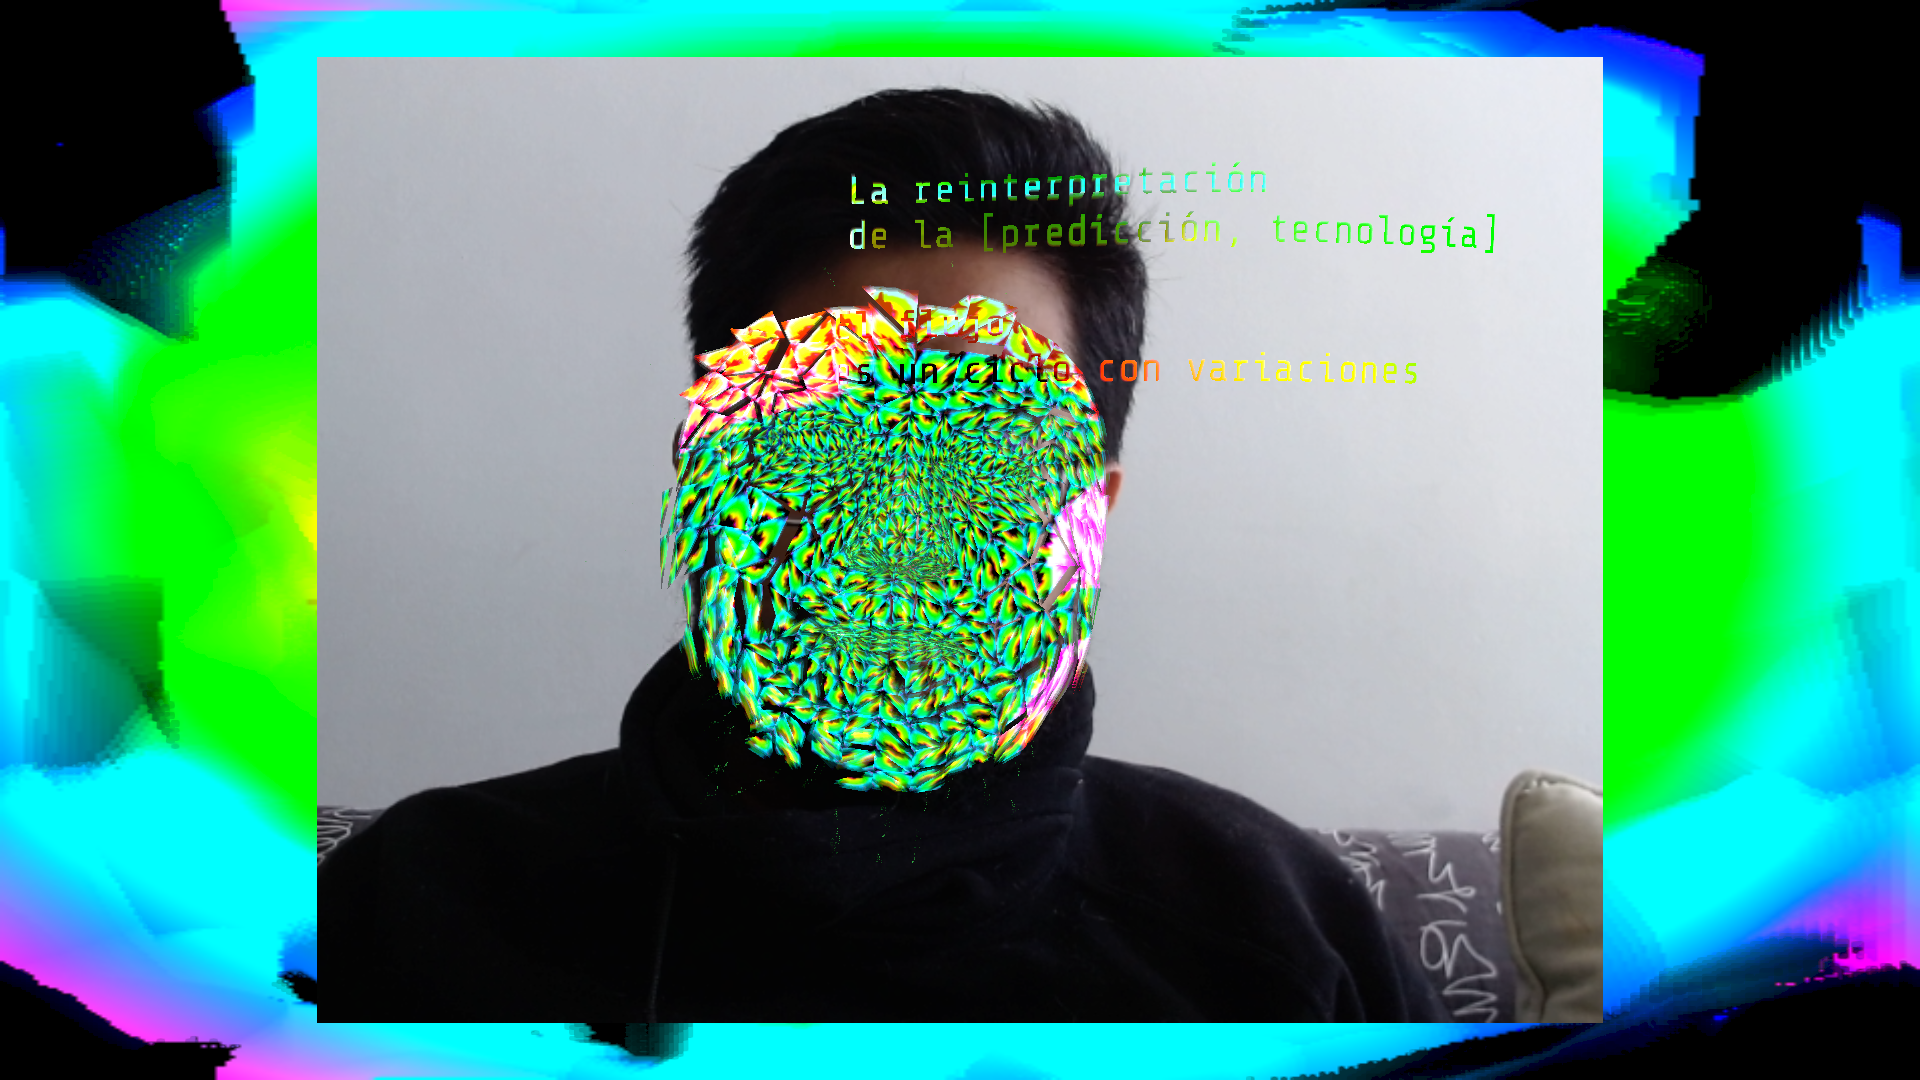
\includegraphics[width=\columnwidth]{../../img/antiHydra2.png} 
\caption[Captura Segunda Versión Anti]{Captura de la segunda versión de Anti}
\label{fig:gallery} 
\end{figure}

\subsection{Mediciones}

Plantear la posibilidad de medir el éxito del proyecto con algoritmos de reconocimiento facial. Dar la vuelta a la tecnología como ofuscación y como posibilidad de éxito frente a esa ofuscación. Mediación del diseño humano, decisiones subjetivas basadas en la experiencia. 

Desde el punto de vista humano ¿existe una retroalimentación adversarial que por un lado alimenta la base de datos que un sistema una computadora utiliza y que como parte de un continuo que no se interrumpe, se alimenta y se ve cuestionado / reforzado en cada iteración? ¿

\section{La escritura como rodeo} % Otra palabra que no sea rodeo 

Resultados y giros. 
Distinción entre investigación / práctica artística y manifiesto 
Escritura de código.

% Texto académico vs && || manifiesto 

Desplazamiento del sonido 

%\subsection{Planteamiento Inicial}
%\subsection{Proceso y realización}
%\subsection{Resultados}
